%Paul E. West

%\documentclass[xcolor=svgnames]{beamer}
\documentclass{beamer}
\usepackage[boxed,vlined,figure]{algorithm2e}

%\usecolortheme[named=FireBrick]{structure}
%\usecolortheme[named=black]{structure}
%\usecolortheme{beetle}
%\usecolortheme{beaver}
%\usecolortheme{crane}
%\usecolortheme{dolphin}
%\usecolortheme{dove}
%\usecolortheme{fly}
%\usecolortheme{lily}
\usecolortheme{orchid}
%\usecolortheme{rose}
%\setbeamercolor{background canvas}{bg=Gold!25}
%\setbeamercolor{background canvas}{bg=Black!100}
%\setbeamercolor{foreground}{bg=Gold!25}
%\setbeamercolor{normal text}{fg=green,bg=black}
%\setbeamercolor*{palette primary}{use=structure,fg=green,bg=black}

\mode<presentation>{
    \usetheme{Darmstadt}
    \setbeamercovered{invisible}
    %\setbeamercovered{transparent}
    \setbeamercolor*{palette primary}{use=structure,fg=white,bg=blue}
    \setbeamercolor*{palette secondary}{use=structure,fg=white,bg=blue}
    \setbeamercolor*{palette tertiary}{use=structure,fg=white,bg=blue}
}

\usepackage[english]{babel}
\usepackage[latin1]{inputenc}
\usepackage{times}
\usepackage[T1]{fontenc}
%\usepackage{epsfig}
\usepackage{ulem}
\usepackage{color,soul}

\usepackage{graphicx}
\usepackage{amssymb}
\usepackage{url,hyperref}
\definecolor{beamer@blendedblue}{rgb}{1,.6,.2}
%\usepackage{tikz}
%\usetikzlibrary{shapes}
%\usetikzlibrary{arrows}
%\tikzstyle{block}=[draw opacity=0.7, line width=1.4cm]
\usepackage{listings}
\lstset{language=C++}
\lstset{showspaces=false}
\lstset{showstringspaces=false}
\lstset{tabsize=4}
\lstset{basicstyle=\tiny}


%\usecolortheme[overlystylish]{albatross}
%\usecolortheme[]{lily}
%\usecolortheme[]{albatross}
%\usecolortheme[]{orchid}
%\setbeamercolor{normal text}{fg=green!10}

\title{CSCI 315: Data Structures}
\author{Paul E. West, PhD}

\institute{
  Department of Computer Science\\
  Charleston Southern University
}

\subject{Software Programming}
%\keywords{Performance Counters, Multicore}

%\pgfdeclareimage[height=1.0cm]{university-logo}{../imgs/csu-logo}
\pgfdeclareimage[height=0.75cm]{university-logo}{../imgs/csu-logo}
%\pgfdeclareimage[height=0.50cm]{university-logo}{../imgs/csu-logo}
\logo{\pgfuseimage{university-logo}}

\begin{document}

\begin{frame}
  \titlepage
\end{frame}

\section{Linux Philosophy}
\subsection{}
\begin{frame}{Linux File Structure}
\begin{itemize}
\item In Linux, everything is a file. Well, almost!
\item Programs can use disk files, serial ports, printers, and other devices in exactly the same way they would use a file.
\item A file has a name and some properties, or ``administrative information''
\item creation/modification date 
\item its permissions
\item The properties are stored in the file's inode
\item a special block of data in the file system
\item contains administrative information
\item contains the length of the file
\item where on the disk it's stored
\end{itemize}
\end{frame}

\begin{frame}{Directories}
\begin{itemize}
\item Directories are files.
\item A directory is a file that holds the inode numbers and names of other files.
\item Each directory entry is a link to a file's inode; remove the filename and you remove the link.
%\item You can see the inode number for a file by using ln -i.
\item If the number of links to a file reaches zero, the inode and the data it references are no longer in use and are marked as free.
\item This allows deletion when there are multiple links to the same file to be managed correctly.
\end{itemize}
\end{frame}

\begin{frame}{Directories continued}
\begin{itemize}
\item Files are arranged in directories, which may also contain sub-directories
\item The / directory sits at the top of the hierarchy and contains all of the system's files in sub-directories
\item The /home directory is a sub-directory of the root directory which is the home of all users
\item /bin for system programs (``binaries'')
\item /etc for system configuration files,
\item /lib for system libraries
\item /dev for physical devices and provide the interface to those devices
\end{itemize}
\end{frame}

\begin{frame}{}
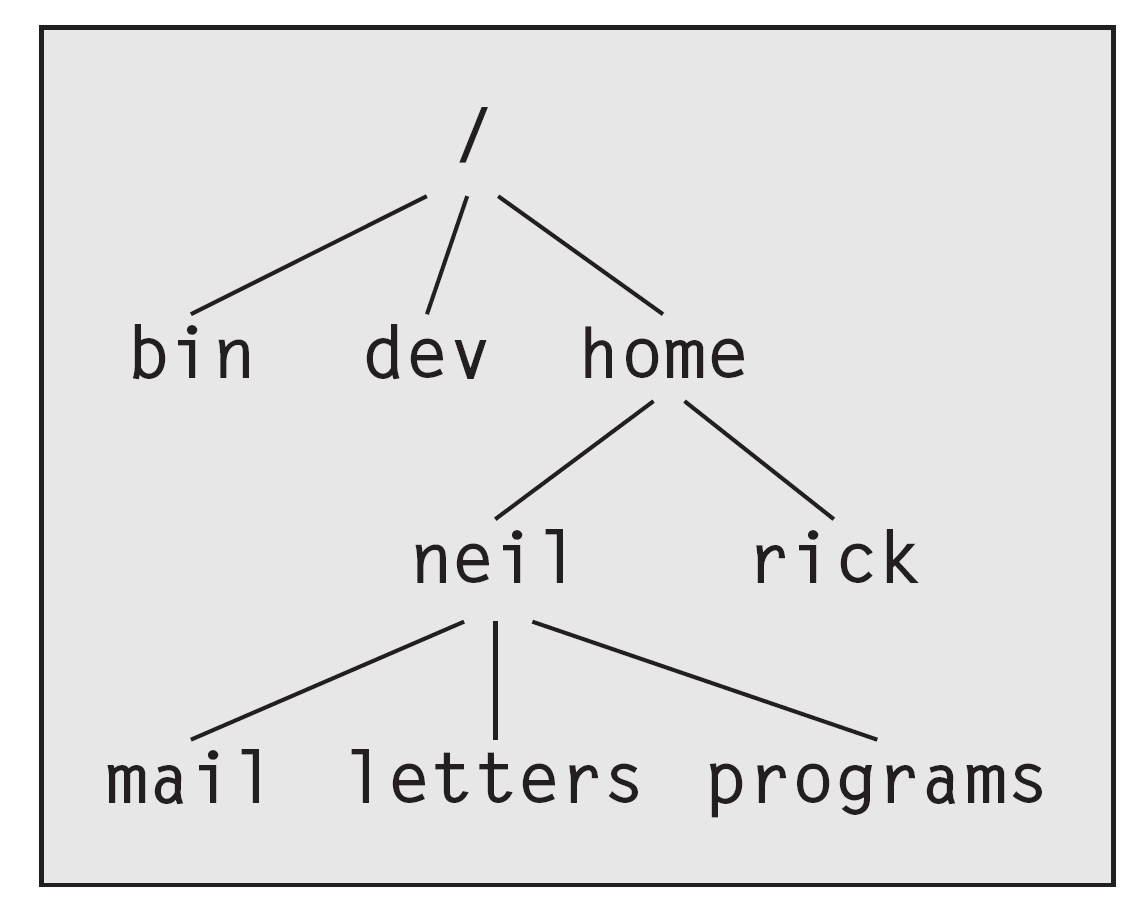
\includegraphics[width=1.0\textwidth]{../imgs/simple-directories.png}
\end{frame}

\begin{frame}{Files and Devices}
\begin{itemize}
\item Even hardware devices are very often represented (mapped) by files.
\item You can mount a CD-ROM drive as a file:
\item \# mount -t iso9660 /dev/hdc /mnt/cdrom
\item \# cd /mnt/cdrom
\end{itemize}
\end{frame}

\begin{frame}{/dev/console}
\begin{itemize}
\item This device represents the system console
\item Error messages and diagnostics are often sent to this device.
\item On Linux, it's usually the ``active'' virtual console
\end{itemize}
\end{frame}

\begin{frame}{/dev/tty}
\begin{itemize}
\item The special file /dev/tty is an alias for the controlling terminal of a process
\begin{itemize}
\item keyboard
\item screen
\item window
\end{itemize}
\item /dev/tty allows a program to write directly to the user, without regard to which pseudo-terminal or hardware terminal the user is using
\end{itemize}
\end{frame}

\begin{frame}{/dev/null}
\begin{itemize}
\item This is the null device.
\item All output written to this device is discarded.
\item Unwanted output (aka a student's email complaint/rant) is often redirected to /dev/null.
\item echo do not want to see this >/dev/null
\item cp /dev/null empty\_file
\end{itemize}
\end{frame}

\section{tmux}
\subsection{}
\begin{frame}
\begin{itemize}
\item tmux: terminal multiplexer
\item This allows us to attach multiple users to the same terminal or to background processes.
\item For this class we will use it to program as a group or to help everyone follow along.
\item How to connect:
\begin{enumerate}
\item First, everyone must be on the CSU \textit{wired} network.
\item I will post the IP address in class.
\item Then ssh over to that IP address (you can use putty if you are in Windows.)
\item login is student/student
\item Then at the command line type: \\
\$ tmux att
\item to exit: ctrl + b and then d.
\end{enumerate}
\end{itemize}
\end{frame}

\section{Compilation}
\subsection{}
\begin{frame}{Introduction}
\begin{itemize}
\item As a programmer or system administrator, you should know how to program under Linux
\item We are going to learn 
\begin{itemize}
\item how to compile a program under Linux (gcc)
\item how to debug (gdb \& ddd)
\item how to automate compilation (make)
\item how to perform memory analysis (valgrind)
\item how to create performance graphs (gnuplot - next set of slides.)
\item how to determine performance issues (perf - if we get to it.)
\end{itemize}
\end{itemize}
\end{frame}

\begin{frame}[fragile]{Compiling under C/C++}
\begin{columns}[c]
\column{0.50\textwidth}
\begin{itemize}
\item We start with the simple case of all your source code in a single file.
\item Try to generate a .c (NOT a .cpp) file as listed on the right hand side.
\end{itemize}
\column{0.50\textwidth}
\begin{lstlisting}
#include <stdio.h>

int main(int argc, char* argv[]) {

    printf("hello world\n");

    return 0;
}
\end{lstlisting}
\end{columns}
\end{frame}

\begin{frame}{Compile}
\begin{itemize}
\item gcc test.c 
\item What file is generated?
\item Name your compiled file by using
\item gcc test.c -o test
\item Run the generated executable file
\end{itemize}
\end{frame}

\begin{frame}{Creating Debug Ready Code}
\begin{itemize}
\item cc -g test.c -o test
\item The '-g' flag tells the compiler to use debug info
\item The compile file size is much larger
\item We may still remove this debug information using the strip command 
\item strip test
\end{itemize}
\end{frame}

\begin{frame}{Adding Optimizations}
\begin{itemize}
\item The compiler can help improve the performance of your code via optimizations
\item cc -O test.c -o test
\item The '-O' flag tells the compiler to optimize the code. 
\item Usually can define an optimization level by adding a number to the '-O' flag
\end{itemize}
\end{frame}

\begin{frame}{Getting Extra Compiler Warnings}
\begin{itemize}
\item Error messages
\begin{itemize}
\item Erroneous code that does not comply with the C standard 
\end{itemize}
\item Warnings 
\begin{itemize}
\item Codes that usually tend to cause errors during runtime 
\end{itemize}
\item Extra compiler warnings 
\begin{itemize}
\item useful to improve the quality of our source code
\item expose bugs that will really bug us later  
\end{itemize}
\item cc -Wall test.c -o test
\end{itemize}
\end{frame}

\begin{frame}[fragile]{Compiling a C++ program}
\begin{lstlisting}
#include <iostream> 

int main(int argc, char* argv[]) {
    std::cout << "hello world" << endl; 
    return 0; 
}
\end{lstlisting}
\end{frame}

\begin{frame}{Compiling Multi Source Programs}
\begin{itemize}
\item compile them
\begin{itemize}
\item cc main.c a.c b.c -o hello\_world
\end{itemize}
\item Comments
\begin{itemize}
\item external symbols need ``extern'' keyword
\item source file order becomes important
\item as program size increases so does compilation time
\end{itemize}
\end{itemize}
\end{frame}

\begin{frame}{Limitation}
\begin{itemize}
\item Even if we only make a change in one of the source files, all of them will be re-compiled when we run the compiler again.
\item To overcome:
\begin{itemize}
\item cc -c main.cc 
\item cc -c a.c 
\item cc -c b.c 
\item cc main.o a.o b.o -o hello\_world 
\end{itemize}
\item ``-c'' tells compiler only to create an object file, and not to generate a final executable file just yet
\item The fourth command links the 3 object files into an executable file
\end{itemize}
\end{frame}

\section{Makefile}
\subsection{}

\begin{frame}{Automating Program Compilation}
\begin{itemize}
\item makefile is a collection of instructions that should be used to compile your program.
\item Once you modify some source files, and type the command ``make'' (or ``gmake'' if using GNU's make), your program will be recompiled using as few compilation commands as possible.
\end{itemize}
\end{frame}


\begin{frame}[fragile]{Makefile Structure}
\begin{itemize}
\item Variable Definitions 
\begin{itemize}
\item define values for variables for reuse\\
\begin{lstlisting}
CFLAGS = -g -Wall 
SRCS = main.c file1.c file2.c 
CC = gcc 
\end{lstlisting}
\end{itemize}
\item Dependency Rules 
\begin{itemize}
\item define under what conditions a given file needs to be re-compiled, and how to compile it. \\
\begin{lstlisting}
main.o: main.c
[tab]        gcc -g -Wall -c main.c 
\end{lstlisting}
\item if any of the files after : change, 
\item then recompile
\item Note: You must use tabs in makefiles! (Spaces will NOT work.)
\item \# is a comment
\end{itemize}
\end{itemize}
\end{frame}

\lstset{language=make}

\begin{frame}[fragile]{Single Source Makefile Example}
\begin{lstlisting}
# first you list your variable(s)
CC = gcc
# top-level rule to create the program. 
# typically top rule is all (by convention)
all: main 
# compiling the source file, main.o depends on main.c
main.o: main.c 
        $(CC)  -g -Wall -c main.c 
# $(CC) uses value of CC variable, case sensitive
# linking the program, program name is main
main: main.o 
        ($CC) -g main.o -o main 
# cleaning everything that can be automatically recreated with "make". 
# basically objects, the executable, and temp files
clean: 
        rm -f main main.o
\end{lstlisting}
\end{frame}

\begin{frame}[fragile]{Multi Source file Example}
\begin{lstlisting}
# top-level rule to compile the whole program. 
all: prog 
# program is made of several source files. 
prog: main.o file1.o file2.o 
        gcc main.o file1.o file2.o -o prog 
# rule for file "main.o". 
main.o: main.c file1.h file2.h 
        gcc -g -Wall -c main.c 
# rule for file "file1.o". 
file1.o: file1.c file1.h 
        gcc -g -Wall -c file1.c 
# rule for file "file2.o". 
file2.o: file2.c file2.h 
        gcc -g -Wall -c file2.c 
# rule for cleaning files generated during compilations. 
clean: 
        rm -f prog main.o file1.o file2.o
\end{lstlisting}
\end{frame}

\begin{frame}{Multi Source Make}
\begin{itemize}
\item Commands can be anything, though usually they are gcc/g++ to compile or link
\item Commands can be multiline, use tabs
\item Other tools:
\begin{itemize}
\item makedepend: Finds dependencies for your program.
\item configure: Finds libraries your program make need.
\end{itemize}
\item We are going to focus only on make for this class.
%\item make param:
%\begin{itemize}
%\item Runs the dependency for param
%\item No param runs first label found (usually all)
%\item make clean deletes files created by make
%\end{itemize}
\end{itemize}
\end{frame}

%\begin{frame}[fragile]{makedepend}
%\begin{itemize}
%\item Program to generate dependencies
%\item Parameters are C/C++ files to scan
%\item It processes \# directives to check includes
%\item Dependencies are critical, can do dependency graphs
%\item Can be added to Makefile:\\
%\begin{lstlisting}
%depend: Makefile $(SRC) 
        %makedepend $(INCLUDES) $(SRC) 
%## end of Makefile 
%# DO NOT DELETE THIS LINE -- make depend depends on it. 
%
%\end{lstlisting}
%\item Now make depend will run makedepend and add its results directly to Makefile.  It doesn't generate the commands, but it does take care of finding dependencies for you.  
%\item Many compilers automatically run dependency checks every time-never misses a dependency, but wasted work
%\end{itemize}
%\end{frame}

%\begin{frame}{configure}
%\begin{itemize}
%\item Configure is part of the autoconf GNU system
%\item It makes Makefiles (ha!)
%\item Finds things (like say tcl) and updates Makefile variables with their locations
%\item Good for multi-platform Makefiles
%\item Not needed for this class
%\end{itemize}
%\end{frame}

\section{Debugging}
\subsection{}

\begin{frame}{Debugging C/C++ Prrograms}
\begin{itemize}
\item Before invoking the debugger, make sure you compiled your program with the "-g" flag (for gcc or g++) \\
gcc -g debug\_me.c -o debug\_me \\
gdb debug\_me
\end{itemize}
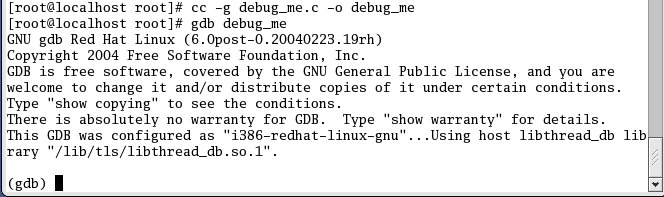
\includegraphics[width=1.0\textwidth]{../imgs/gdb1.png}
\end{frame}

\begin{frame}{Quitting}
\begin{itemize}
\item q quits the debugger
\item Only do this when you are done, not when you want to reload a program
\end{itemize}
\end{frame}

\begin{frame}{Running the Program Inside a Debugger}
\begin{itemize}
\item Once we invoked the debugger, we can run the program using the command "run".
\item Can also just use the single letter r
\item If the program requires command line parameters, we can supply them to the "run" command of gdb \\
run "hello, world" "goodbye, world"
\end{itemize}
\end{frame}

\begin{frame}{Setting Breakpoints}
\begin{itemize}
\item A break point is a command for the debugger to stop the execution of the program before executing a specific source line. 
\item Specifying a specific line of code to stop in: \\
break 9		(assumes only 1 source file)\\
break debug\_me.c:9\\
   debug\_me.c is the file name, 9 is the line number\\
\item Specifying a function name, to break every time it is being called: \\
break main 			OR\\
b main
\item Can also give a Boolean expression for conditional breakpoints
\end{itemize}
\end{frame}

\begin{frame}{list}
\begin{itemize}
\item list \#\\
Shows that line number and next few lines\\
Hit return to show more lines\\
Can also just use letter l\\
\item l debug\_me:\#
\end{itemize}
\end{frame}

\begin{frame}{Stepping A Command At A Time}
\begin{itemize}
\item Type command\\
break main \\
run "hello, world" "goodbye, world"
\end{itemize}
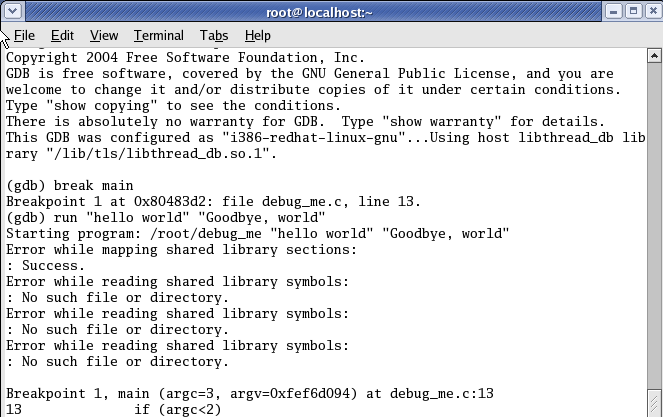
\includegraphics[width=0.7\textwidth]{../imgs/gdb2.png}
\end{frame}

\begin{frame}{Stepping A Command At A Time (continued...)}
\begin{itemize}
\item Now we want to start running the program slowly, step by step. 
\item "next" (or n) - (step over) execute the current command, and stop again, showing the next command in the code to be executed. 
\end{itemize}
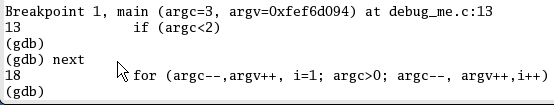
\includegraphics[width=1.0\textwidth]{../imgs/gdb3.png}
\end{frame}

\begin{frame}{Stepping A Command At A Time (continued...)}
\begin{itemize}
\item step (or s) - (step into functions) execute the current command, and if it is a function call - break at the beginning of that function 
\item step \# - step \# number of steps
\end{itemize}
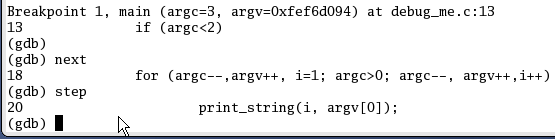
\includegraphics[width=1.0\textwidth]{../imgs/gdb4.png}
\end{frame}

\begin{frame}{Printing Variables And Expressions}
\begin{itemize}
\item print (or p) the contents of a variable with a command like this: 
\begin{itemize}
\item print i \\
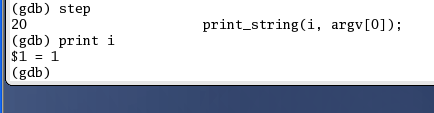
\includegraphics[width=0.8\textwidth]{../imgs/gdb5.png}
\end{itemize}
\item You may also try to print more complex expressions, like "i*2", or "argv$[$3$]$", or "argv$[$argc$]$"
\end{itemize}
\end{frame}

\begin{frame}{Examining The Function Call Stack}
\begin{itemize}
\item Once we got into a break-point and examined some variables, we might also wish to see "where we are". 
\item This can be done using the "where" command 
\end{itemize}
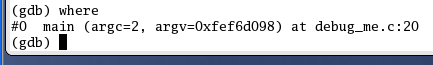
\includegraphics[width=1.0\textwidth]{../imgs/gdb6.png}
\end{frame}

\begin{frame}{Examining The Function Call Stack}
\begin{itemize}
\item we can see contents of variables local to the calling function, or to any other function on the stack \\
frame 1 \\
print i  
\item The "frame" command tells the debugger to switch to the given stack frame
\item "0" is the frame of the currently executing function. 
\end{itemize}
\end{frame}

\begin{frame}{Debugging A Crashed Program}
\begin{itemize}
\item Sometimes a program is will generate a core file containing its memory image when it crashes 
\item May also use backtrace (bt) shows series of functions calls to where we are
\item Once we get such a core file, we can look at it by issuing the following command \\
gdb /path/to/program/debug\_me core 
\end{itemize}
\end{frame}

\begin{frame}{Miscellaneous}
\begin{itemize}
\item When you type run, it checks if executable has changed, but doesn't do recompilation
\item kill terminates currently running code, but doesn't exit gdb
\item help (or h) gives general help
\item Help command gives help on some command
\end{itemize}
\end{frame}

\begin{frame}{ddd}
\begin{itemize}
\item GUI wrapper for gdb
\item Also a wrapper for Java's jdb, Perl's and Python's pdb, among others
\item apt-get install ddd
\end{itemize}
\end{frame}

\section{Sys Arch}
\subsection{}

\begin{frame}{System Calls And Device Drivers}
\begin{itemize}
\item We can access and control files and devices using system calls
\item At the heart of the operating system, the kernel, are a number of device drivers.
\item The low-level functions used to access the device drivers, the system calls, include:
\begin{itemize}
\item open: Open a file or device
\item read: Read from an open file or device
\item write: Write to a file or device
\item close: Close the file or device
\item ioctl: Pass control information to a device driver
\end{itemize}
\end{itemize}
\end{frame}

\begin{frame}{System Calls And Device Drivers}
\begin{itemize}
\item The problem with using low-level system calls directly for input and output is that they can be very inefficient.
\item Why?
\begin{itemize}
\item Performance penalty in making a system call.
\item The hardware has limitations
\end{itemize}
\item To provide a higher-level interface to devices and disk files, provides a number of standard libraries
\end{itemize}
\end{frame}

\begin{frame}{}
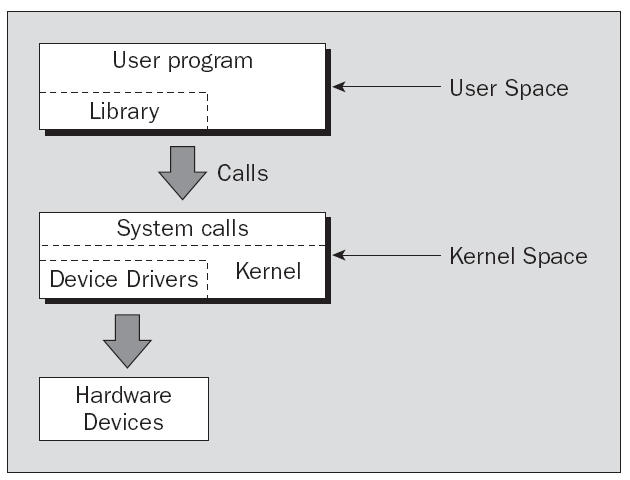
\includegraphics[width=1.0\textwidth]{../imgs/sys-arch.png}
\end{frame}

\section{Valgrind}
\subsection{}

\begin{frame}{What Even Is?}
\begin{itemize}
\item A tool to perform
\begin{itemize}
\item memory debugging
\item memory leak detection
\item memory profiling
\end{itemize}
\item Valgrind accomplishes this by running your program inside of its virtual machine and capturing all your memory accesses/requests.
\end{itemize}
%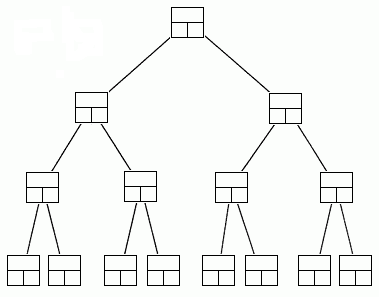
\includegraphics[width=1.0\textwidth]{../imgs/binary-tree.png}
\end{frame}

\begin{frame}[fragile]{Memory debugging}
\begin{itemize}
\item A successful run:
\end{itemize}
\begin{lstlisting}
==2231== Memcheck, a memory error detector
==2231== Copyright (C) 2002-2013, and GNU GPL'd, by Julian Seward et al.
==2231== Using Valgrind-3.10.0 and LibVEX; rerun with -h for copyright info
==2231== Command: ./a.out
==2231== 
==2231== 
==2231== HEAP SUMMARY:
==2231==     in use at exit: 0 bytes in 0 blocks
==2231==   total heap usage: 0 allocs, 0 frees, 0 bytes allocated
==2231== 
==2231== All heap blocks were freed -- no leaks are possible
==2231== 
==2231== For counts of detected and suppressed errors, rerun with: -v
==2231== ERROR SUMMARY: 0 errors from 0 contexts (suppressed: 0 from 0)
\end{lstlisting}
\begin{itemize}
\item Notice Valgrind keeps track of:
\begin{itemize}
\item (heap) memory used on exit
\item How much heap memory was allocated \& freed
\item How many memory errors (out of bounds memory access) were detected.
\end{itemize}
\item The ``2231'' is the process id, which for this class is unimportant
\end{itemize}
\end{frame}

\begin{frame}[fragile]{Memory Leak Detection}
\begin{itemize}
\item Let's examine an obvious memory leak:
\end{itemize}
\begin{lstlisting}
int main(int argc, char *argv[]) {
    int *ints = new int[1024];

    return 0;
}
\end{lstlisting}
g++ test.c \&\& valgrind ./a.out
\begin{lstlisting}
==2476== HEAP SUMMARY:
==2476==     in use at exit: 4,096 bytes in 1 blocks
==2476==   total heap usage: 1 allocs, 0 frees, 4,096 bytes allocated
==2476== 
==2476== LEAK SUMMARY:
==2476==    definitely lost: 4,096 bytes in 1 blocks
==2476==    indirectly lost: 0 bytes in 0 blocks
==2476==      possibly lost: 0 bytes in 0 blocks
==2476==    still reachable: 0 bytes in 0 blocks
==2476==         suppressed: 0 bytes in 0 blocks
\end{lstlisting}
\begin{itemize}
\item Definitly lost means ... we lost ...
\item Inderectly lost means, we lost and it could be hard to find.
\item Possibly lost means Valgrind was not able to determine if the memory was deallocated or not.
\item Still reachable means you have a dangling pointer(more later).
\end{itemize}
\end{frame}

\begin{frame}[fragile]{Memory Usage detection}
\begin{itemize}
\item A better version:
\end{itemize}
\begin{lstlisting}
int main(int argc, char *argv[]) {
    int *ints = new int[1024];

    delete[] ints;
    return 0;
}
\end{lstlisting}
g++ test.c \&\& valgrind ./a.out
\begin{lstlisting}
==2591== HEAP SUMMARY:
==2591==     in use at exit: 0 bytes in 0 blocks
==2591==   total heap usage: 1 allocs, 1 frees, 4,096 bytes allocated
==2591== 
==2591== All heap blocks were freed -- no leaks are possible
\end{lstlisting}
\begin{itemize}
\item Notice Valgrind can tell us how much heap memory we are using even though we freed (deallocated) it.
\end{itemize}
\end{frame}

\begin{frame}[fragile]{Memory Access Error Detection}
\begin{itemize}
\item Now lets use Valgrind to detect a off by one memory error.
\end{itemize}
\begin{lstlisting}
int main(int argc, char *argv[]) {
    int *ints = new int[1024];

    for (int i = 0; i <= 1024; i++) {
        ints[i] = i;
    }

    delete[] ints;
    return 0;
}
\end{lstlisting}
Do you see the error?
\begin{lstlisting}
==2615== Invalid write of size 4
==2615==    at 0x400673: main (in /home/pwest/t/a.out)
==2615==  Address 0x5a03040 is 0 bytes after a block of size 4,096 alloc'd
==2615==    at 0x4C298A0: operator new[](unsigned long) (vg_replace_malloc.c:389)
==2615==    by 0x40064E: main (in /home/pwest/t/a.out)
==2615== 
==2615== 
==2615== HEAP SUMMARY:
==2615==     in use at exit: 0 bytes in 0 blocks
==2615==   total heap usage: 1 allocs, 1 frees, 4,096 bytes allocate
\end{lstlisting}
\begin{itemize}
\item Well that tells us the error, but where is it?
\end{itemize}
\end{frame}

\begin{frame}[fragile]{Getting A Little More Help}
\begin{itemize}
\item Compile with debug flags! (g++ \textit{-g} test.c \&\& valgrind ./a.out)
\end{itemize}
\begin{lstlisting}
==2634== Invalid write of size 4
==2634==    at 0x400673: main (test.c:7)
==2634==  Address 0x5a03040 is 0 bytes after a block of size 4,096 alloc'd
==2634==    at 0x4C298A0: operator new[](unsigned long) (vg_replace_malloc.c:389)
==2634==    by 0x40064E: main (test.c:4)
==2634== 
==2634== 
==2634== HEAP SUMMARY:
==2634==     in use at exit: 0 bytes in 0 blocks
==2634==   total heap usage: 1 allocs, 1 frees, 4,096 bytes allocated
==2634== 
==2634== All heap blocks were freed -- no leaks are possible
\end{lstlisting}
\end{frame}

\begin{frame}{Conclusion}
\begin{itemize}
\item Valgrind can be used to detect memory leaks and memory access errors.
\item Valgrind provides other tools to profile memory usage and cache usage, but those are beyond the scope of this class.
\item Notice that Java has memory debugging built it, but C++ doesn't.  Why?
\end{itemize}
\end{frame}

\section{Future}
\subsection{}

\begin{frame}{Other Tools}
\begin{itemize}
%\item gprof: Used to profile
%\begin{itemize}
%\item Profiling tells you where you program is spending the most time.
%\item With that knowledge you can focus you energy on certain parts to speed up performance.  (Why?)
%\end{itemize}
\item gnuplot: Generates simple graphs
\begin{itemize}
\item gnuplot plugs in nicely with how we do things
\item You may use something else, if you *really* want too...
\end{itemize}
\item perf (hopefully)
%\item Before gprof and gnuplot, we need to learn Bash!
\end{itemize}
\end{frame}

\end{document}
